\part{Rotating field theory}
\title[Rotating field theory]{Rotating field theory}  
\date{}  
\frame{\titlepage} 

%%%%%%%%%%%%%%%%%%%%%%%%%%%%%%%%%%%%%%%%%%%%%%%%%%%%%%%%%%%%%
%% Conceptual idea of a rotating magnetic field %%
%%%%%%%%%%%%%%%%%%%%%%%%%%%%%%%%%%%%%%%%%%%%%%%%%%%%%%%%%%%%%
\begin{frame}
	\frametitle{Conceptual idea of a rotating magnetic field}
    \begin{figure}
        \centering
        \movie{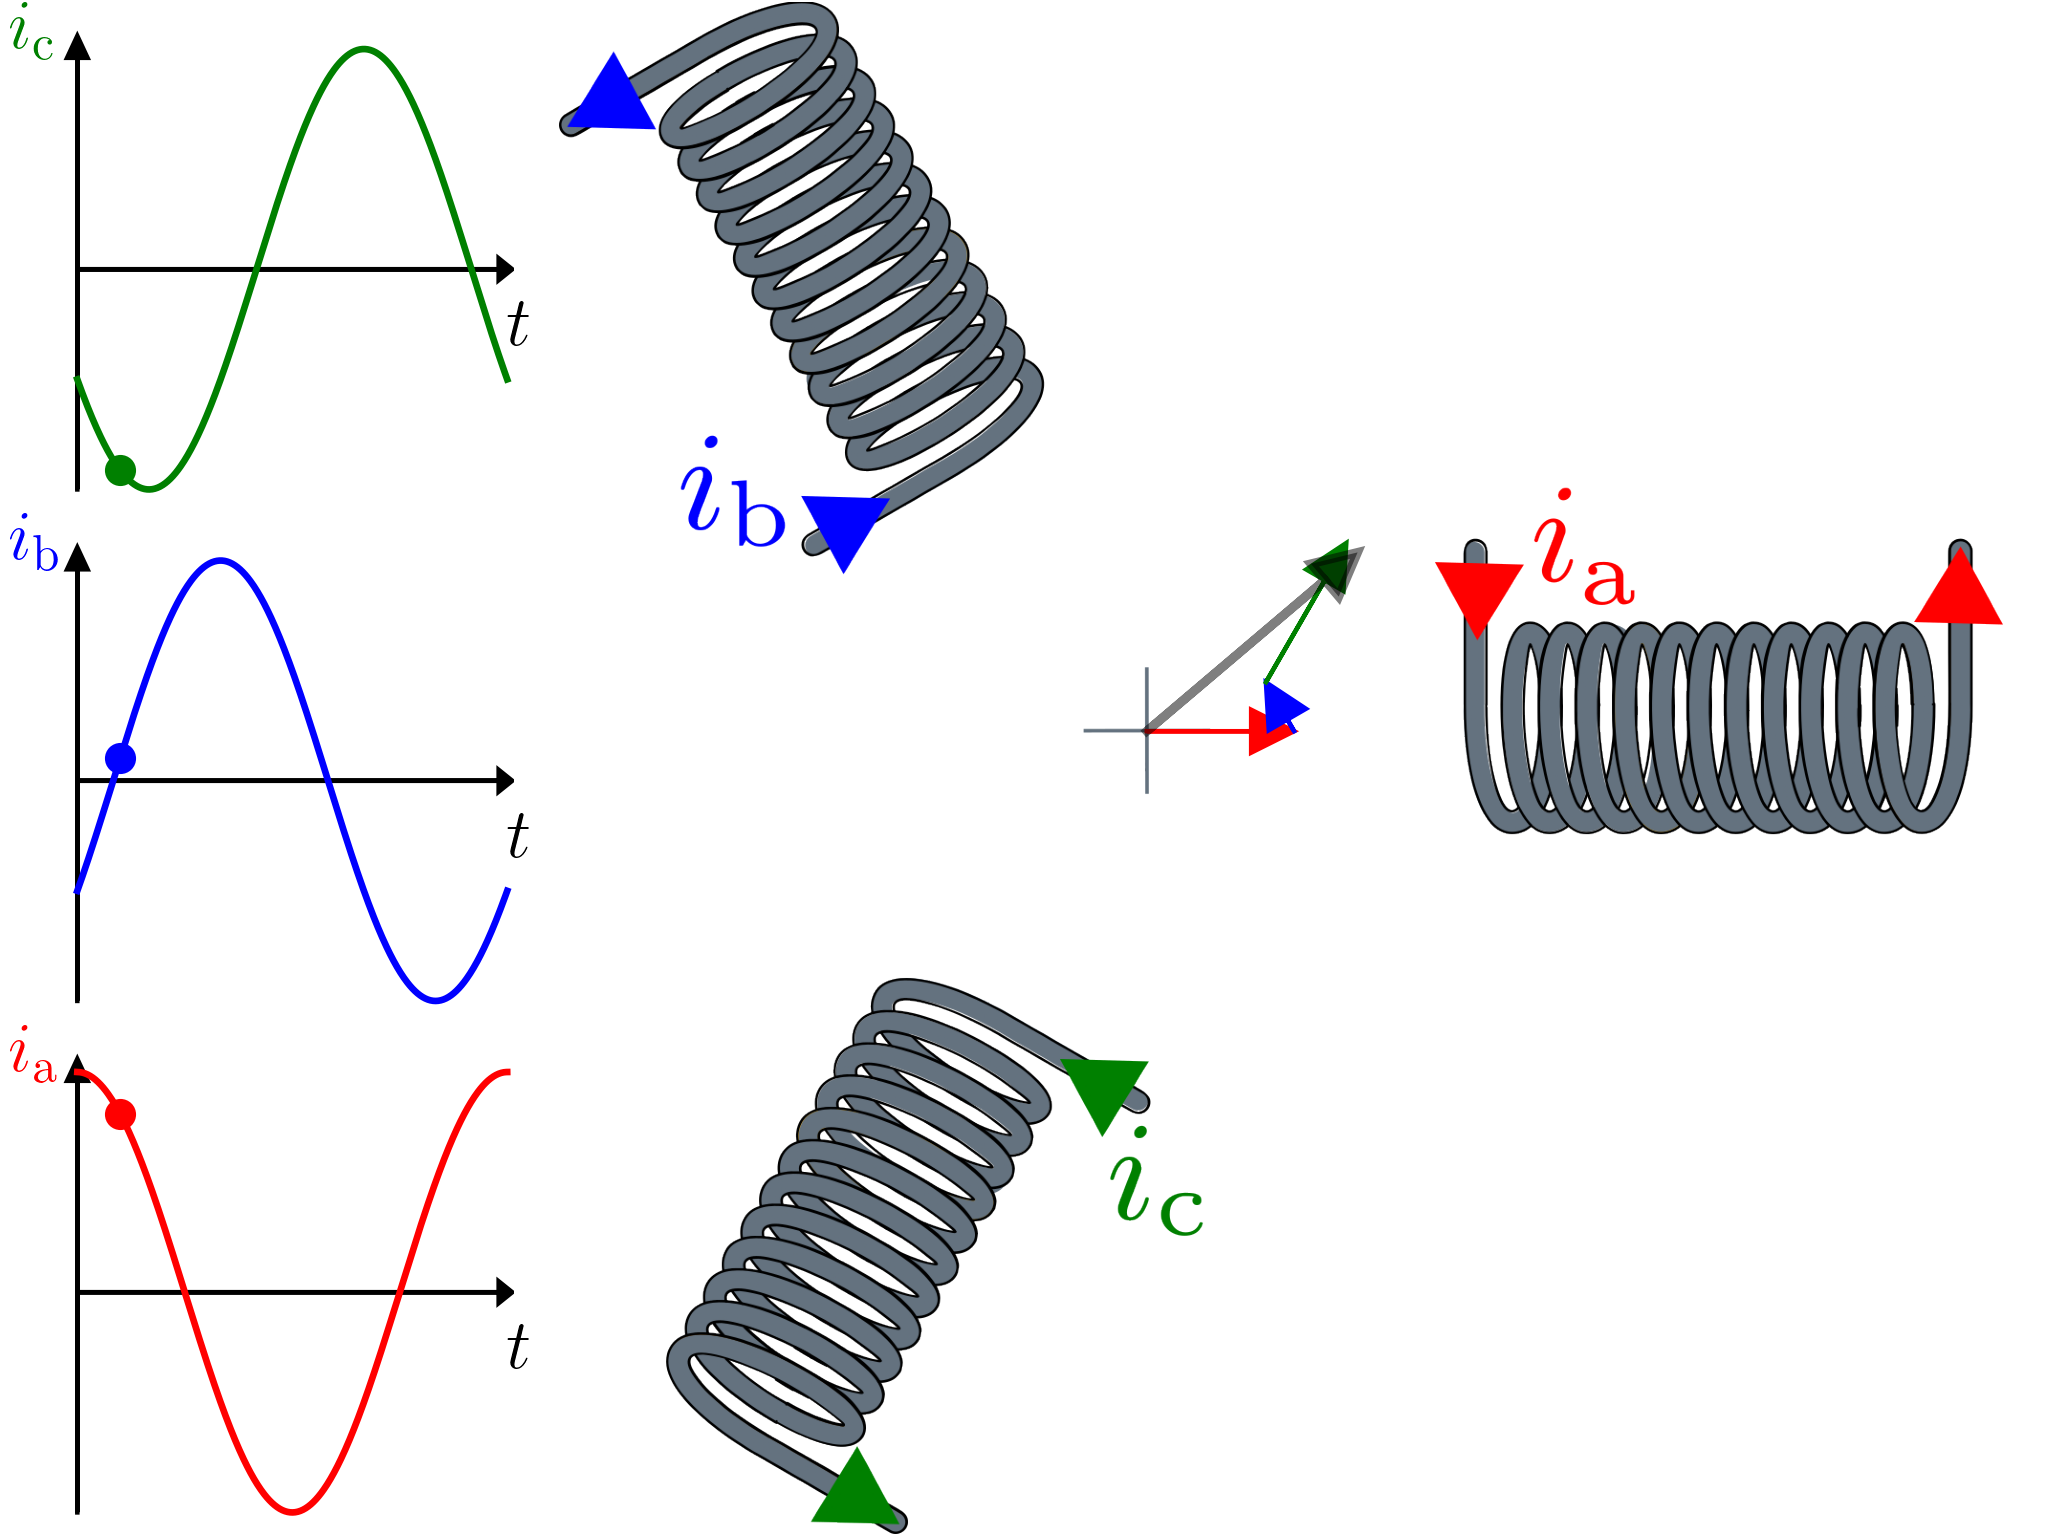
\includegraphics[height=0.7\textheight]{fig/lec05/Three_phase_coils_rotating_field_preview.png}}{fig/lec05/Three_phase_coils_rotating_field.gif}
        \caption{Animation of a rotating magnetic field produced by three-phase currents in three coils both physically and electrically displaced by $120^\circ$ (inspired by \href{https://perso.univ-lyon1.fr/charles.joubert/web_anim/simen_rotfield_create.html}{C.~Joubert})}
    \end{figure}
\end{frame}

%%%%%%%%%%%%%%%%%%%%%%%%%%%%%%%%%%%%%%%%%%%%%%%%%%%%%%%%%%%%%
%% Basic rotating field model %%
%%%%%%%%%%%%%%%%%%%%%%%%%%%%%%%%%%%%%%%%%%%%%%%%%%%%%%%%%%%%%
\begin{frame}
	\frametitle{Basic rotating field model}
    \begin{columns}
		\begin{column}{0.55\textwidth}
	        We assume an ideal three-phase stator current:
            \begin{equation}
                \begin{split}
                    i_\mathrm{s,a}(t) &= \hat{i}_{\mathrm{s}} \cos(\omega t), \\
                    i_\mathrm{s,b}(t) &= \hat{i}_{\mathrm{s}} \cos(\omega t - 2\pi/3), \\
                    i_\mathrm{s,c}(t) &= \hat{i}_{\mathrm{s}} \cos(\omega t + 2\pi/3).
                \end{split}
            \end{equation}
            The index 's' indicates stator quantities, but is omitted in the following as we will only consider stator quantities until further notice, i.e.,, 
            $$i_\mathrm{s,a}(t) = i_\mathrm{a}(t), \quad i_\mathrm{s,b}(t) = i_\mathrm{b}(t), \quad i_\mathrm{s,c}(t) = i_\mathrm{c}(t)$$
            and $\hat{i}_{\mathrm{s}}=\hat{i}$. 
        \end{column}
        \begin{column}{0.45\textwidth}
            \begin{figure}
                \centering
                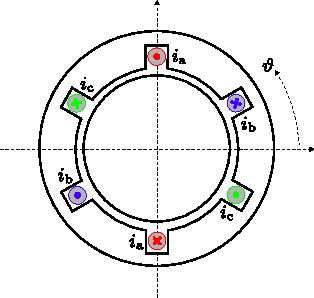
\includegraphics[width=0.8\textwidth]{fig/lec05/Simple_three_phase_stator_lumped_coils.pdf}
                \caption{Elementary three-phase stator winding with lumped coils  displaced by $120^\circ$. The rotor is considered an unspecific solid dummy with very high magnetic permeability.}
                \label{fig:Simple_three_phase_stator_lumped_coils}
            \end{figure}
        \end{column}
    \end{columns}
\end{frame}